\documentclass[10pt,conference]{IEEEtran}
\IEEEoverridecommandlockouts
% The preceding line is only needed to identify funding in the first footnote. If that is unneeded, please comment it out.
\usepackage{cite}
\usepackage[utf8]{inputenc}
\usepackage[T1]{fontenc}
\usepackage{amsmath,amssymb,amsfonts}
\usepackage{algorithmic}
\usepackage{graphicx}
\usepackage{textcomp}
\usepackage{xcolor}
\usepackage{enumitem}
\usepackage{multirow}
\usepackage{tabularx}
\usepackage{array}
\usepackage{booktabs}
\usepackage{siunitx} % 用于数字对齐
\usepackage{adjustbox} % 新增：用于缩放表格

\def\BibTeX{{\rm B\kern-.05em{\sc i\kern-.025em b}\kern-.08em
    T\kern-.1667em\lower.7ex\hbox{E}\kern-.125emX}}
\begin{document}

\title{Root Cause Analysis of RISC-V Build Failures via LLM and MCTS Reasoning
%\\
%{\footnotesize \textsuperscript{*}Note: Sub-titles are not captured in Xplore and should not be used}

\thanks{Corresponding authors: Jie Liu, Dan Ye. Supported by Strategic Priority Research Program of the Chinese Academy of Sciences (XDA0320102), the National Natural Science Foundation of China (42361144884), Fundamental Research Project of ISCAS (ISCAS-JCMS-202405)}
}


\author{%
\IEEEauthorblockN{Weipeng Shuai\IEEEauthorrefmark{1}\IEEEauthorrefmark{2}, Jie Liu\IEEEauthorrefmark{1}\IEEEauthorrefmark{2}\IEEEauthorrefmark{3}\IEEEauthorrefmark{4}, Zhirou Ma\IEEEauthorrefmark{1}\IEEEauthorrefmark{2}\IEEEauthorrefmark{3}, Liangyi Kang\IEEEauthorrefmark{1}, Zehua Wang\IEEEauthorrefmark{1}\IEEEauthorrefmark{2}, Shuai Wang\IEEEauthorrefmark{1}\IEEEauthorrefmark{2}\\
Dan Ye\IEEEauthorrefmark{1}\IEEEauthorrefmark{2}, Hui Li\IEEEauthorrefmark{1}\IEEEauthorrefmark{2}, Wei Wang\IEEEauthorrefmark{1}\IEEEauthorrefmark{2}\IEEEauthorrefmark{3}\IEEEauthorrefmark{4}, Jiaxin Zhu\IEEEauthorrefmark{1}\IEEEauthorrefmark{2}\IEEEauthorrefmark{3}\IEEEauthorrefmark{4}}
\IEEEauthorblockA{\IEEEauthorrefmark{1}Institute of Software, Chinese Academy of Sciences, Beijing, China}
\IEEEauthorblockA{\IEEEauthorrefmark{2}University of Chinese Academy of Sciences, Beijing, China}
\IEEEauthorblockA{\IEEEauthorrefmark{3}University of Chinese Academy of Sciences, Nanjing, China}
\IEEEauthorblockA{\IEEEauthorrefmark{4}Laboratory of System Software (Chinese Academy of Sciences), Beijing, China}
\IEEEauthorblockA{\{shuaiweipeng22, ljie, mazhirou, kangliangyi15, wangzehua23\}@otcaix.iscas.ac.cn\\
\{wangshuai, yedan, lihui2012, wangwei, zhujiaxin\}@otcaix.iscas.ac.cn}
}

\maketitle

\begin{abstract}
Build failures are a major obstacle in RISC-V software migration, often involving complex interactions across logs, configurations, and environments. Traditional diagnostic tools struggle with the unstructured, multi-phase nature of build logs and lack semantic reasoning.

We propose a two-stage framework for automated root cause analysis. RV-LAD compresses logs using template-based filtering and applies phase-aware anomaly detection via few-shot LLM prompting. MCTS-RCA integrates a domain-specific knowledge base with Monte Carlo Tree Search to perform LLM-guided multi-source reasoning under classification constraints.

To support evaluation, we construct a curated dataset of 117 real-world RISC-V build failures, each annotated with logs, spec files, and repair records. Experiments show our approach achieves 75.2\% diagnosis accuracy, surpassing previous LLM-based and rule-based methods. It also offers interpretable reasoning traces, enabling practical and transparent diagnosis.
This work provides an effective and extensible solution for RCA in emerging software ecosystems like RISC-V, bridging large language models with domain-aware inference.
\end{abstract}

\begin{IEEEkeywords}
Root Cause Analysis, Large Language Model, Log Anomaly Detection, RISC-V Software Migration
\end{IEEEkeywords}

\section{Introduction}

\begin{table*}[htbp]
\centering
\caption{RISC-V Build Error Classification}
\begin{tabularx}{\textwidth}{|>{\bfseries}l|>{\bfseries}l|X|}
\hline
% 标题行居中对齐
\multicolumn{1}{|c|}{\textbf{Error Category}} 
& \multicolumn{1}{c|}{\textbf{Subcategory}} 
& \multicolumn{1}{c|}{\textbf{Description}} \\ 
\hline

\multirow{3}{*}{Dependency Error} 
& Missing Dependency          &-Dependency missing, incorrect version, or incompatible library in build system \\ 
& Dependency Cycle            &-Circular dependency chain preventing resolution and package installation \\
& Dependency Conflict         &-Version requirements clash between packages due to overlapping dependencies \\
\hline

\multirow{2}{*}{Test Failure} 
& Unit Test Failure           &-Package unit tests did not pass with failed assertions or edge cases \\
& Integration Test Failure    &-Cross-component integration tests failed due to interface mismatches \\
\hline

\multirow{3}{*}{Configuration Error} 
& Compatibility Issues        &-Compiler, architecture, API, function signature, or file path compatibility issues \\
& Spec File Misconfiguration&-Invalid/incomplete spec file settings causing build process misbehavior \\
& Environment Variables Missing &-Required variables unset during build leading to undefined behavior \\
\hline

\multirow{4}{*}{Compilation Error} 
& Source Code Errors          &-Syntax/type/logic defects in code including undeclared variables or missing semicolons \\
& API Breaking Changes        &-Code unadapted to dependent library API updates causing linkage failures \\
& Missing Header Files        &-Required headers not located in include paths or dependency chains \\
& Plugin Compilation Failure  &-Plugin build process failed due to missing symbols or invalid interfaces \\
\hline

\multirow{3}{*}{Packaging Error} 
& Resource Missing            &-Critical files/directories not found during build causing incomplete installation \\
& Memory Exhaustion           &-Insufficient memory allocation caused failure in linking or code generation \\
& Timeout Exceeded            &-Execution duration surpassed threshold during long-running compilation tasks \\
\hline

\multirow{2}{*}{Network Error} 
& Source Fetch Failure        &-Repository code download failed due to connection timeouts or authentication issues \\
& Dependency Download Failure &-Library/package retrieval error caused by network instability or proxy restrictions \\
\hline

\end{tabularx}
\end{table*}

% LogCure: Automated Diagnosis of Build Failures in Software Migration to RISC-V Through two-stage log Distillation and Reasoning

In recent years, RISC-V as an open-source, modular and scalable instruction set architecture has catalyzed a paradigm shift in processor design\cite{r1,r4}. Its flexibility in processor design has led to widespread migration of mainstream software packages to RISC-V\cite{r16}. However, a large amount of performance-critical code relies on proprietary instructions (e.g., AES-NI, AVX). As a result, there are frequent build failures during the migration of software packages from other architectures (e.g., x86/ARM), which often lead to missing third-party library adaptations, misconfigured toolchain versions, and so on. These errors delay deployment and require specialized expertise for diagnosis, significantly hindering the maturation of the RISC-V software ecosystem.

The Open Build Service (OBS) platform is a widely adopted platform for building RISC-V software packages. The build process in OBS is highly automated and generates extensive build logs that document the entire migration process to facilitate debugging for developers. While these logs theoretically provide a goldmine for root cause analysis of build errors in software migration, their practical utility is hampered by three inherent challenges. First, the logs span from tens of thousands to hundreds of thousands of lines, with critical error messages buried in less than 5\% of the content. Second, log formats exhibit extreme heterogeneity across software packages and dynamically evolve during build phases (e.g., installation, compilation, packaging). Moreover, the build process in RISC-V packages often exhibit cross-layer coupling, requiring the joint analysis of multi-source heterogeneous information such as abnormal signals in logs, missing declarations in configuration files, and conflicting logic in patch files. Third, error patterns lack standardized keywords that require heuristic rules for preliminary filtering. To address these challenges, Table I presents a systematic categorization of RISC-V build errors into six major classes with corresponding subcategories, providing a structured foundation for subsequent diagnostic analysis.


\begin{figure*}
    \centering
    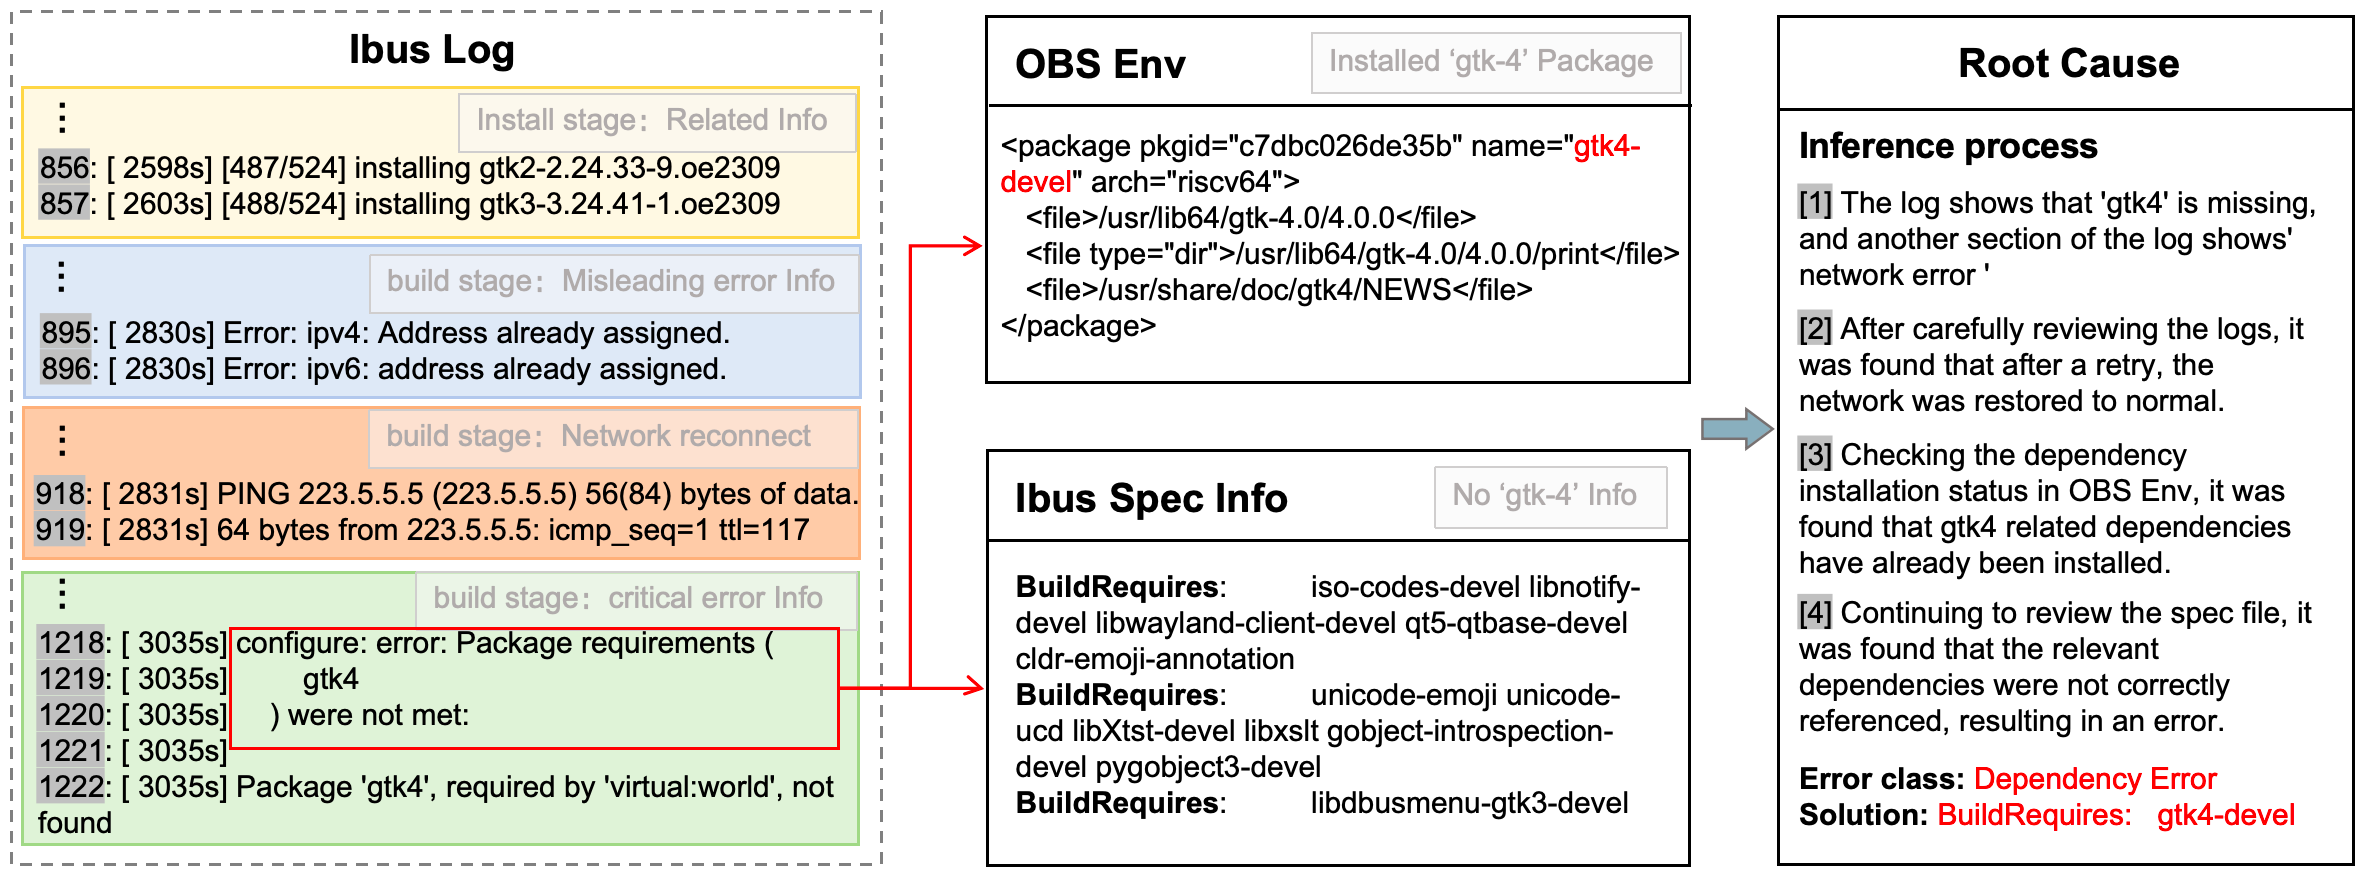
\includegraphics[width=1\linewidth]{pic/ibus-exp-530.png}
    \caption{Workflow for Resolving ibus Build Issues in RISC-V}
    \label{fig:1}
\end{figure*}



Consider the failed build of the \textit{ibus} package in OBS. The initial log analysis in Figure~\ref{fig:1} revealed conflicting clues: Fragment 2 suggested a "network failure" while Fragment 4 indicated a missing \textit{gtk-4} dependency. 
Relying solely on either fragment in isolation would inevitably lead to incorrect root cause attribution -- potentially chasing network ghosts or overlooking the core configuration defect. However, the critical breakthrough came from systematically cross-referencing these signals with crucial artifacts: Fragment 3 (which hints at the reconnection of network), the package's spec file (revealing the absence of gtk4-devel in the BuildRequires section), and the dependency environment within the OBS build worker. This information conclusively exposed the true root cause: an undeclared build dependency on gtk-4 within the package's spec file. 

This example highlights the necessity of integrating multi-source artifacts for accurate diagnosis. Developers must iteratively correlate error signals with configuration parameters and dependency versions, a process that requires architectural expertise and hours of manual effort per failure.

Prior attempts to automate RISC-V build error diagnosis face two critical shortcomings. First, traditional log parsers rely on rigid rule-based or template-matching techniques\cite{r17,r18}, failing to adapt to the format diversity and phase-specific log structures of RISC-V builds. Second, existing tools analyze error signals in isolation (e.g., logs-only or spec file-only), neglecting cross-layer dependencies between compilation errors, dependency conflicts, and configuration mismatches\cite{r12,r14}. For instance, single-source analyzers might misinterpret a "missing header" error as a code defect, overlooking its link to incorrect include paths in the build environment. Nowadays, advanced LLM agents provide new impetus for automatic log analysis. However, directly feeding such logs into large language models (LLMs) may exceed context length limits and lead to a loss of domain knowledge. These limitations stem from an inability to dynamically prioritize evidence sources or perform iterative reasoning, resulting in low diagnostic accuracy.


To overcome these barriers, we propose a two-stage solution combining log compression with multi-source causal reasoning. First, we introduce a phase-aware log anomaly detector that employs template-guided retrieval to compress logs by 92\%, prioritizing error snippets while preserving contextual clues (e.g., timestamps, build stage identifiers). Unlike supervised methods, Template-based minimizes reliance on labeled data by leveraging RISC-V build phase semantics. Second, we devise a \textit{Monte Carlo Tree Search (MCTS)} framework that synergizes large language models (LLMs) with domain knowledge bases and a toolset. This framework dynamically constructs a multi-source evidence reasoning path, guiding LLMs to explore hypotheses through iterative rollouts---simulating human-like reasoning paths. 

We curate a dataset of 117 real-world RISC-V build failures, spanning six error categories: compile problems (18.8\%), dependency issues (38.5\%), build errors (6.8\%), configuration errors (14.5\%), test failures (19.17\%), and network anomalies (1.7\%). Each case includes raw logs, spec files, dependency environment, and verified repair patches. Our framework is instantiated as an \textit{autonomous repair agent} that orchestrates Template-based and MCTS modules, interfacing with OBS to validate fixes through automated rebuilds. Experiments demonstrate an 75.2\% diagnosis accuracy, reducing manual effort by 63\%. The agent's decision traces, visualized as reasoning trees, provide interpretable audit trails for developers---a critical feature for industrial adoption.

This work bridges the gap between LLM-driven automation and domain-specific debugging, offering a scalable pathway to accelerate RISC-V ecosystem maturation. 
This paper makes the following three contributions:

% \begin{figure}
%     \centering
%     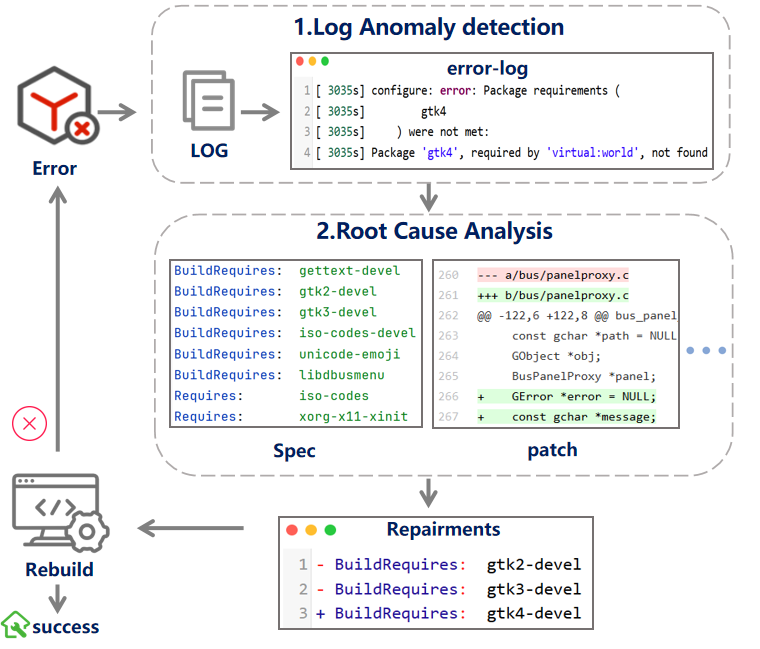
\includegraphics[width=1\linewidth]{pic/human-repair.png}
%     \caption{Manual repair process for build errors}
%     \label{fig:enter-label}
% \end{figure}

%To address the problem of root cause analysis for build errors in RISC-V software packages, this study proposes an automated solution that integrates multi-stage log anomaly detection with deep root cause reasoning. The key contributions of this work are as follows:
\begin{enumerate}
\item 
%We propose progressive Causal Reasoning Framework for RISC-V Build Logs. The template retrieval-augmented generation (TemplateRAG) method constructs a phase-aware dynamic template library for log compression. Integrated with a Monte Carlo Tree Search (MCTS) path-planning mechanism, it simulates human experts' "hypothesis-validation" diagnostic workflow.

We propose RV-LAD, a template-based, phase-aware log anomaly detection method that compresses noisy RISC-V build logs and enables accurate error localization via few-shot LLM prompting.
    
\item We introduce MCTS-RCA, a Monte Carlo Tree Search-based root cause reasoning framework that integrates domain-specific knowledge and LLM-guided multi-hop inference for interpretable diagnosis.
    
\item We construct a curated dataset of 117 real-world RISC-V build failures with multi-source annotations (logs, spec files, repair records), and conduct comprehensive experiments showing that our method significantly outperforms prior LLM- and rule-based baselines in accuracy, fix rate, and transparency.

\end{enumerate}

\section{RELATED WORK}

\subsection{Log Anomaly Detection}

Log Anomaly Detection (LAD) is a critical task in information technology\cite{r5,r6} that aims to identify anomalous log entries or sequences that deviate from normal patterns within massive log data to uncover potential system issues or abnormal behaviors.

Existing LAD methodologies can be categorized into three classes: deep learning-based approaches, semi-supervised methods, and unsupervised methods. Deep learning-based approaches automatically extract temporal, semantic, and topological features from logs via neural networks, overcoming the limitations of traditional rule-based methods\cite{r5}. SigML++\cite{trivedi2023sigml++} proposed a supervised LAD method that used probabilistic polynomial approximations for the modeling of log data. Semi-supervised methods address label scarcity by combining limited labeled data with unsupervised learning strategies. PLElog\cite{yang2021plelog} is an early semi-supervised log anomaly detection method based on probabilistic label estimation. Later, LogALST\cite{wang2024semi} introduced a semi-supervised LAD framework integrating active learning and self-training to mitigate performance degradation caused by insufficient labeled logs. Unsupervised methods rely solely on intrinsic log distribution modeling without requiring labeled data. MAD-GAN\cite{li2019mad} developed a multivariate time-series anomaly detection method based on Generative Adversarial Networks (GAN). However, deep learning-based LAD methods face challenges such as dependency on large-scale labeled data or high-quality pretraining, poor interpretability due to model opacity, and limited generalization to dynamic log formats.

Large Language Models (LLMs) offer new opportunities for automated anomaly diagnosis by effectively capturing subtle differences between normal and anomalous patterns, while their few-shot learning capabilities alleviate high annotation costs and class imbalance issues in log data\cite{guan2024logllm}. Recent works like ADUL\cite{hadadi2024anomaly} proposed a fine-tuned LLM-based method to address detection failures caused by frequent log format changes in continuous integration environments. LLMeLog\cite{he2024llmelog} introduced a knowledge-enhanced hierarchical fine-tuning framework focusing on semantic representations of log events. LogGPT\cite{qi2023loggpt} constructed an end-to-end detection framework based on ChatGPT, with core innovations in knowledge-augmented prompting and multimodal response generation. However, existing methods lack phase-awareness and RISC-V-specific error lexicons, resulting high false negatives in RISC-V-specific errors. Our Template-based addresses this by integrating build-stage semantics.

\begin{figure*}
    \centering
    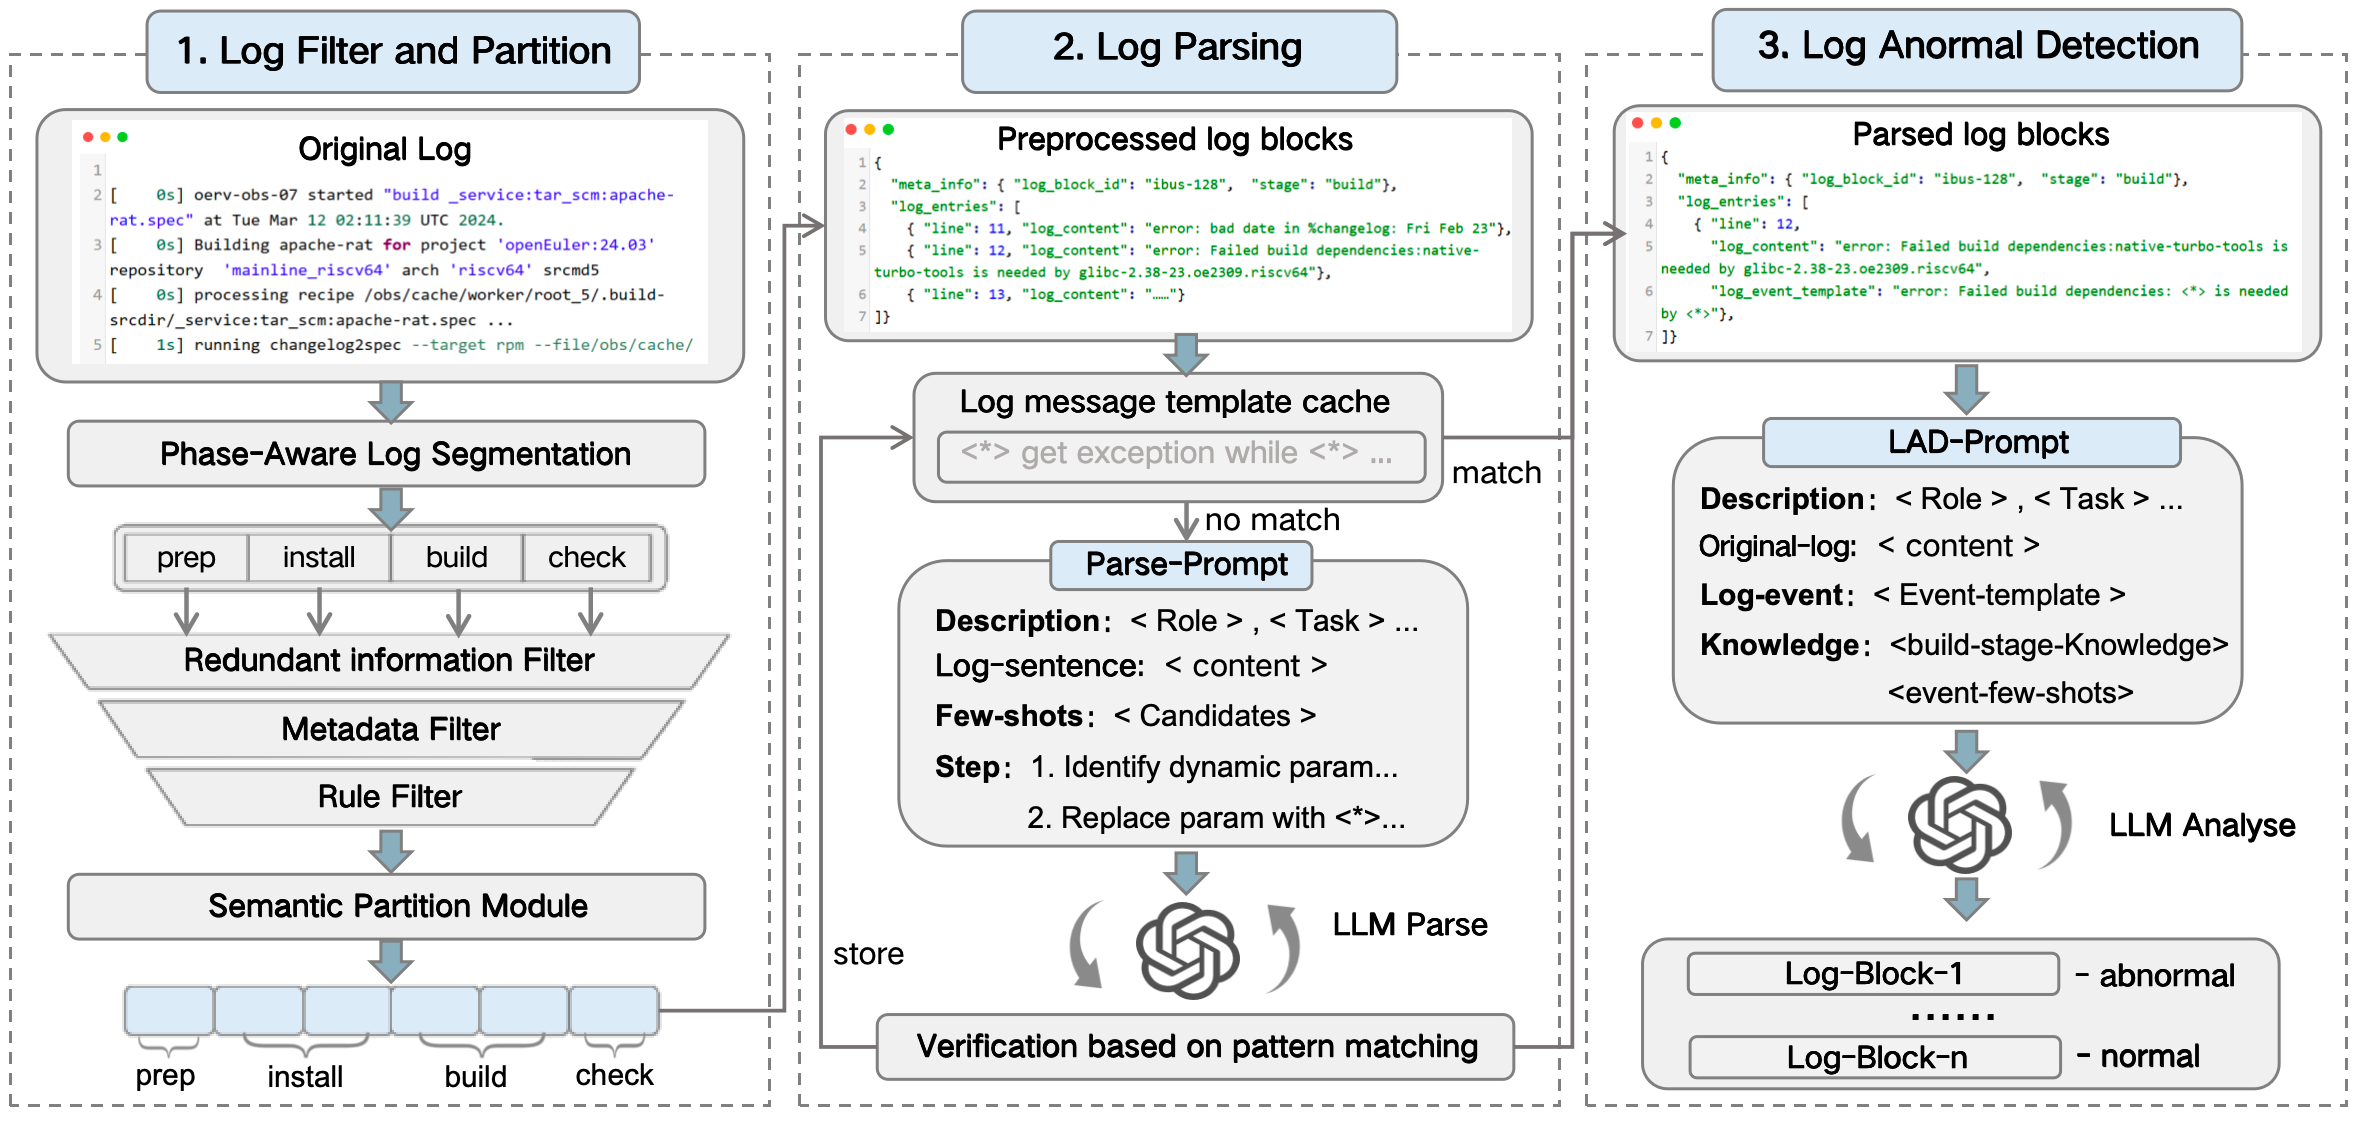
\includegraphics[width=1\linewidth]{pic/lad-530.png}
    \caption{Phase-Aware Log Anomaly Detection via Log Templates for RISC-V Architecture}
    \label{fig:lad}
\end{figure*}

\subsection{Root Cause Analysis}
Root Cause Analysis (RCA) is a critical process to identify the underlying causes of system failures or abnormal behaviors\cite{zhong2024debug,xu2024unilog}. 

Traditional RCA methods mainly rely on the extracted features of the data analysis to pinpoint the root causes. Squeeze\cite{li2019generic} proposed a multidimensional root cause localization method based on large-scale multidimensional data, which efficiently located root causes in a large-scale search space through a "bottom-up and then top-down" search strategy. LogMaster\cite{fu2012logmaster} exploited apriori-like algorithms to extract correlations of events that have multiple attributions. LogMine\cite{hamooni2016logmine} works in iterative manner that generates a hierarchy of patterns (regexes), one level at every iteration. The hierarchy provides flexibility to users to select the right set of patterns that satisfies their specific needs. Later, machine learning-based approaches automate the extraction of knowledge from complex data relationships but require substantial training data and suffer from poor model interpretability. For instance, FluxRank\cite{liu2019fluxrank} is a widely deployable framework for automated fault localization in software services. MSCRED\cite{zhang2019deep} proposed a deep neural network model that enables unsupervised anomaly detection and diagnosis in multivariate time-series data. Although these algorithms effectively discover potential causal associations, they face limitations in interpretability and sensitivity to data quality.

With the rapid advancement of large-scale deep learning models and natural language processing, LLM-based RCA methods have emerged as a pivotal research direction in software maintenance. LogLlama\cite{yang2025logllama} input the raw logs into LLMs for causal inference. However, it overlooks cross-artifact validation leading to hallucinated hypotheses. PACE-LM\cite{zhang2023pace} is a calibrated confidence estimation framework that combines LLMs augmented by prompting and retrieval for RCA events in the cloud. LogKG\cite{sui2023logkg} is a new framework for diagnosing failures based on knowledge graphs of logs, which extracts entities and relations from logs to mine multi-field information and their relations through the KG. But it is not suitable for heterogeneous RISC-V build logs. Recent work like RCAgent\cite{wang2024rcagent} proposed a tool-augmented LLM autonomous agent framework for root cause analysis in cloud environments. However, current tools lack iterative reasoning across logs, configs, and dependency graphs. Our MCTS framework bridges this by simulating human-like multi-step validation.


\section{ METHODOLOGY}

%\subsection{Overview}\label{AA}
We adopt a concise two-stage pipeline for diagnosing RISC-V build failures. Stage I (RV-LAD) performs phase-aware log distillation: it segments logs by build phase, filters noise, parses parameter-agnostic templates, and ranks anomalous snippets via few-shot LLM prompting, outputting top-k snippets with phase, timestamp, and chunk metadata. Stage II (MCTS-RCA) consumes these structured snippets together with spec files, environment metadata, and a RISC-V knowledge base. An LLM proposes hypotheses and tool calls while Monte Carlo Tree Search verifies and selects reasoning paths, producing the final root cause with an interpretable trace and supporting evidence. 

\subsection{RV-LAD: RISC-V Log Anomaly Detection}\label{sec:lad}
To mitigate semantic interference and retrieval bias, we propose RV-LAD---a template-based, phase-aware log anomaly detection method. It first filters and partitions build logs with multi-heuristic rules, then parses parameter-agnostic event templates via real-time semantic parsing, and finally injects phase-specific knowledge into the templates so LLMs can detect stage-aware anomalies. As illustrated in Figure~\ref{fig:lad}, RV-LAD comprises three phases: (1) Log Filtering \& Partition---heuristic filtering and semantic segmentation; (2) Log Parsing---decouple static patterns from dynamic parameters to form templates; (3) Template-based Anomaly Detection---use knowledge-augmented prompts for precise localization.


\subsubsection{Log Filtering and Partition}\label{ss:lad-filter}
In the first phase, the complete software package build log is segmented into phase-specific log chunks. Multi-heuristic rules are then applied to filter out irrelevant information, while excessively long log sequences undergo semantic chunking. This approach enables subsequent anomaly detection to incorporate phase-specific contextual information, effectively addressing the challenge of log structural heterogeneity.

The phase begins by designing multi-heuristic log filtering rules to retain critical diagnostic elements while removing redundant information from log files, providing high signal-to-noise ratio inputs for downstream dynamic prompting mechanisms. The filtering mechanism incorporates three complementary strategies: (1) Redundant Information Filters eliminate repetitive content (e.g., duplicate lines, verbose paths) through similarity hashing and pattern recognition; (2) Metadata Filters preserve critical contextual markers (e.g., phase identifiers, temporal boundaries) to maintain diagnostic provenance; (3) Rule-based Filters apply domain-specific heuristics (e.g., compiler error thresholds, build-stage patterns) to selectively retain semantically meaningful content. Additionally, log chunking serves as a crucial processing step that divides lengthy log files into semantically coherent chunks based on semantic correlations between log statements. This strategy not only reduces the context length requirements for single LLM inference (e.g., through dynamic overlapping mechanisms to ensure inter-chunk semantic continuity) but also preserves metadata (e.g., phase identifiers, timestamp ranges) to establish clear localization references for subsequent root cause analysis.

After filtering and semantic chunking, the RISC-V software package build logs are transformed into structured JSON-formatted log chunks. These chunks contain rich semantic information and metadata, establishing essential preconditions for subsequent anomaly detection.

\begin{figure*}
    \centering
    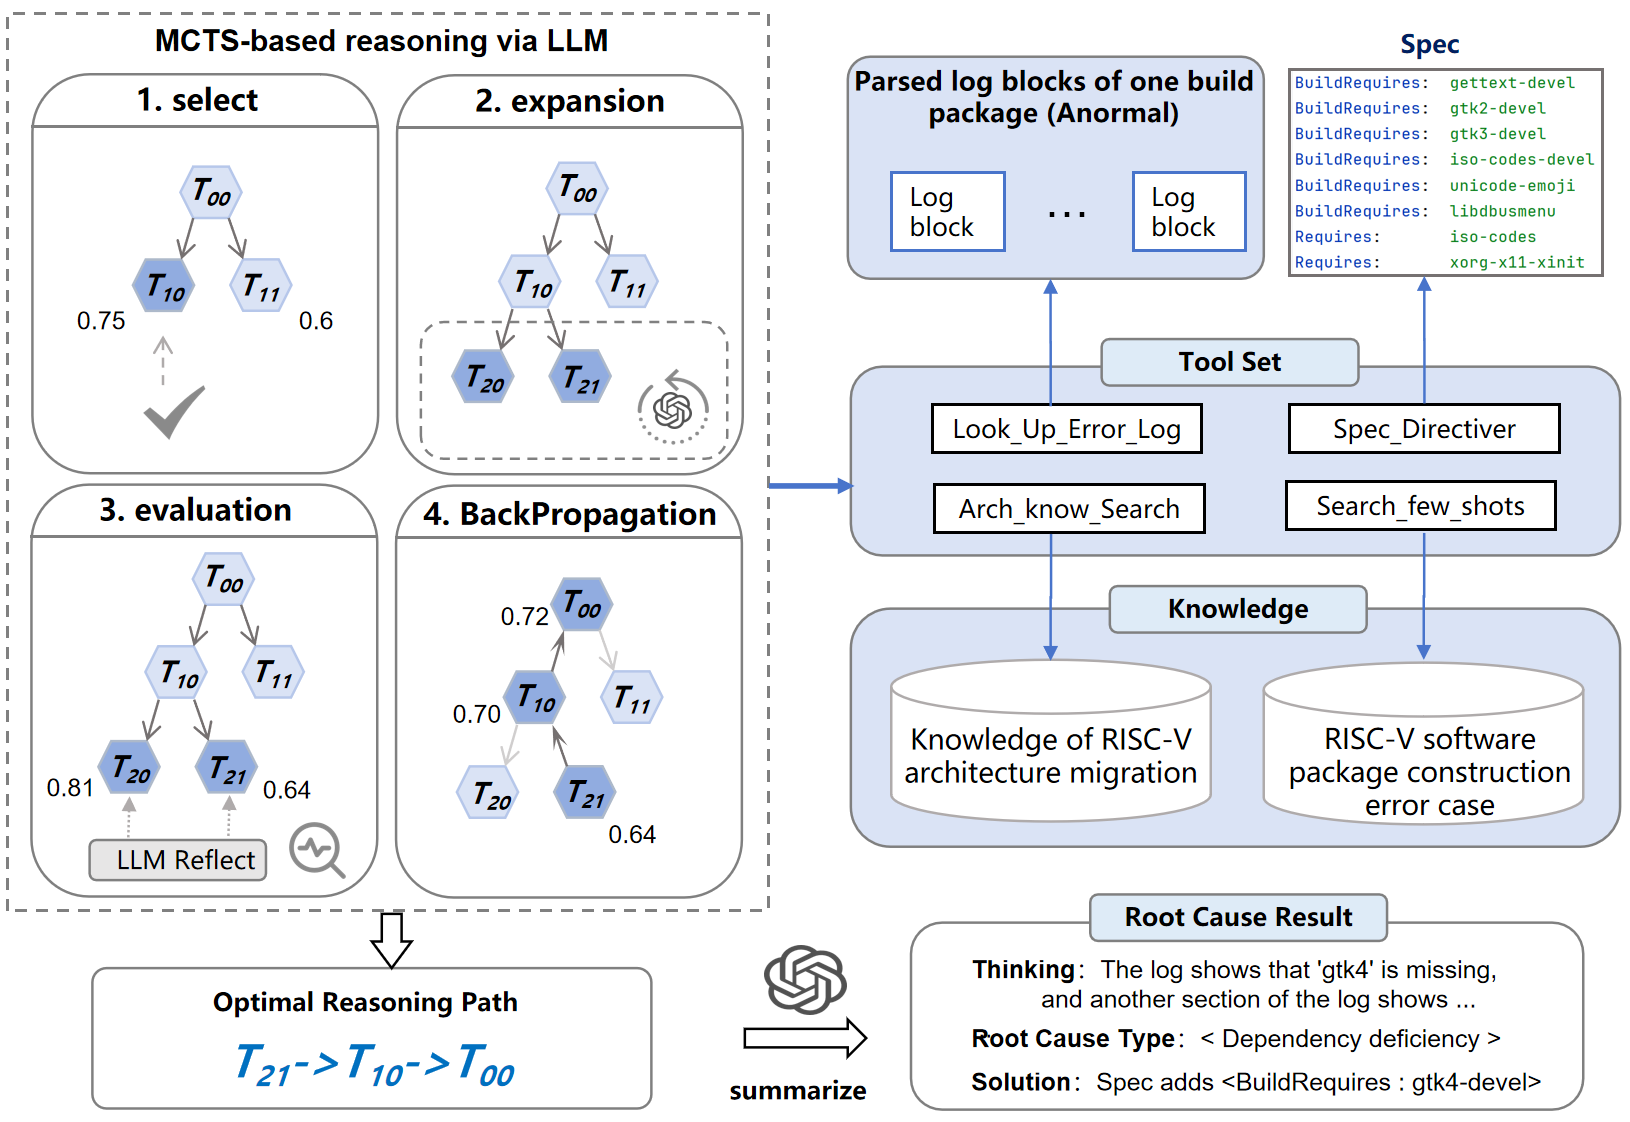
\includegraphics[width=0.8\linewidth]{pic/new-mcts-liu.png}
    \caption{A MCTS-Driven Inference Framework for Root Cause Identification in RISC-V Architecture}
    \label{fig:mcts-overview}
\end{figure*}

\subsubsection{Log Parsing}\label{ss:lad-parsing}
Traditional log parsing methods (e.g., regular expressions, clustering algorithms) exhibit significant limitations when processing RISC-V software package build logs, particularly in handling nested parameters and multi-language dynamic outputs. Leveraging the semantic comprehension and text generation capabilities of large language models (LLMs), this paper proposes an LLM-based real-time log parsing method. It dynamically generates log templates through LLMs’ semantic understanding and reuses historical parsing results via a caching mechanism. Empirical evidence shows that the number of unique log templates in real systems is orders of magnitude smaller than log message volumes. For instance, the Loghub-2.0 dataset contains over 50 million log messages but fewer than 3,500 unique templates. Based on this observation, our method introduces an event template caching mechanism that skips redundant parsing for recurring log events by storing parsed templates. Only cache-missed samples trigger model-based parsing. To ensure parsing consistency, the cache employs a dynamic update strategy: newly generated templates via in-context learning (ICL)-enhanced parsing are optimized through semantic alignment and parameter generalization (e.g., replacing variables with wildcards like "*" to maintain template standardization and reusability.

The core workflow begins with cache matching , where input log statements are compared against cached templates. If a match is found, parsing is skipped to avoid redundancy. For unmatched logs, candidate sampling is performed by selecting representative log messages from the cache based on positional metadata and semantic similarity. These candidates and templates are integrated into a structured prompt during the prompt construction phase, which serves as input to the LLM. The LLM subsequently generates log templates in the LLM-based parsing phase, leveraging its contextual learning capabilities. Finally, a log template validation module verifies the semantic integrity and structural correctness of the generated templates to ensure reliability.


\subsubsection{Template-Based Anomaly Detection}\label{ss:lad-template}
In the third phase, this method proposes a multi-stage dynamic prompting strategy that embeds domain knowledge into phase-specific prompt templates to guide large language models (LLMs) in accurately identifying stage-aware anomaly patterns. Specifically, dedicated prompt templates are designed for each build phase, integrating phase-specific summarization knowledge (e.g., typical error code lists, common dependency conflict patterns) and log syntax rules (e.g., regular expression patterns) during dynamic prompt construction. This enhancement strengthens the LLM’s ability to comprehend contextual semantics.

As shown in Figure~\ref{fig:lad}, to achieve precise LLM guidance, this study constructs structured prompts based on the RISEN framework , aligning instructions through role definition, task decomposition, and format constraints. Domain knowledge, such as similar log cases and phase-specific rules, is embedded into prompts during construction. After prompt finalization, the system inputs the prompts to the LLM, which generates log anomaly detection results. The LLM returns true if it identifies error information in the current log chunk and false otherwise. By combining phase-specific knowledge, adjacent log event templates, raw log content, and parsed templates, this approach significantly improves the efficiency and accuracy of log anomaly detection, providing high-quality inputs for subsequent root cause analysis.


\subsection{MCTS-RCA}\label{sec:mcts}

The Monte Carlo Tree Search-Based Root Cause Analysis Method(MCTS-RCA) aims to enhance diagnostic efficiency and accuracy for RISC-V software build errors through the integration of structured search strategies and domain knowledge. The method consists of two core phases: the offline preparation phase and the online root cause analysis phase, as shown in Figure~\ref{fig:mcts-overview}. In the offline preparation phase, the primary objective is to construct a domain knowledge base and toolkit for root cause analysis, enabling the LLM to dynamically acquire relevant contextual information during diagnosis. The online root cause diagnosis phase employs a collaborative reasoning framework combining Monte Carlo Tree Search (MCTS) and LLM-driven inference. Its central goal is to identify the optimal root cause hypothesis by iteratively exploring and evaluating multi-step decision paths.

\subsubsection{Knowledge Base Construction}\label{ss:mcts-kb}

\begin{figure}
    \centering
    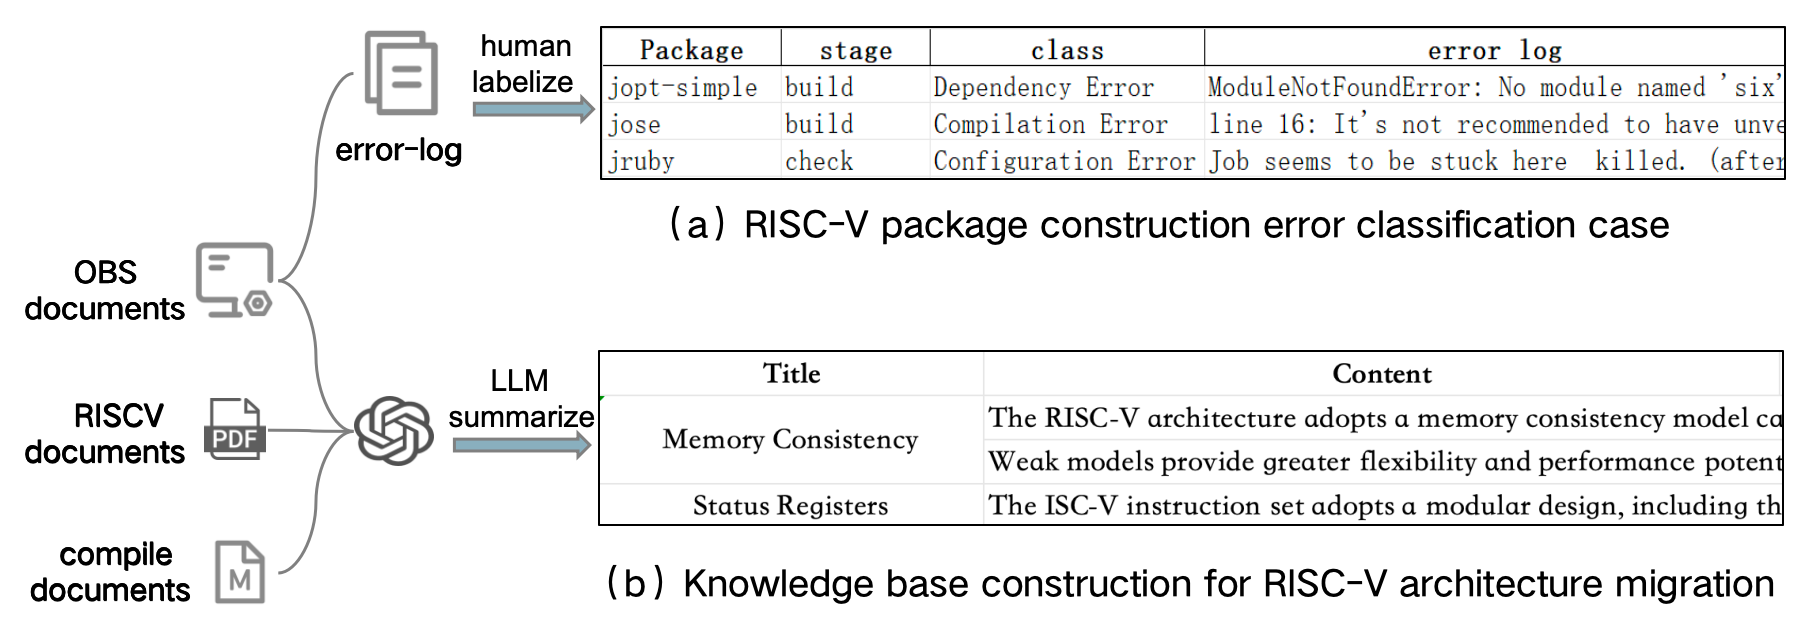
\includegraphics[width=1\linewidth]{pic/knowledge-530.png}
    \caption{Schematic diagram of knowledge base construction}
    \label{fig:mcts-kb}
\end{figure}

Offline knowledge bases include two types: RISC-V architecture migration knowledge base and RISC-V software package construction log error classification case knowledge base. 

The RISC-V architecture migration knowledge base includes common issues and solutions for RISC-V software package migration. The RISC-V software package construction log error case knowledge base comes from real data in the OBS production environment, involving more than 3000 construction tasks. After professional screening and annotation, a historical case knowledge base containing 2940 abnormal records was finally formed. As shown in Figure 4 (a), each record is stored in CSV format, including software package name, error stage, error log content, and predefined error categories (such as missing dependencies, incompatible architecture instructions, etc.), forming a semi-structured case knowledge base that provides rich historical references for subsequent root cause analysis.

As shown in Figure 4 (b), to construct the RISC-V knowledge base, we began by systematically collecting and integrating various knowledge documents pertaining to the RISC-V platform. Secondly, we extracted structured knowledge regarding build processes from the OBS (Open Build Service) platform. Concurrently, we analyzed relevant code commit histories and issue tracking logs on the Gitee platform to acquire practical knowledge concerning code revisions, bug fixes, and feature optimizations.
Subsequently, all the multi-source information gathered and organized—including technical documentation, build process knowledge, and records from code commits and issue tracking—was uniformly fed into a Large Language Model (LLM). We leveraged the LLM's robust summarization and learning capabilities to enable it to identify and distill RISC-V-specific knowledge that was either scarce or not covered in its pre-existing training data. This refined, specialized knowledge was ultimately organized into a standardized JSON format document.
The resulting JSON document serves as the foundation of the RISC-V domain-specific knowledge base. This knowledge base is clearly structured and contains specialized content, designed for efficient invocation by LLMs in subsequent tasks to provide more precise and expert support related to RISC-V.



\subsubsection{ToolSet Construction}\label{ss:mcts-tools}

LLM-based agents need to obtain relevant knowledge and information feedback in real time through tool calls to accurately and efficiently complete root cause analysis tasks. Specifically, the toolset mainly includes the following four types of tools:
\begin{enumerate}
\item Spec file parsing tool: This tool aims to extract key configuration information from the. spec file during the RISC-V software package construction process, providing LLM with configuration information such as build phase instructions and dependencies.
    
\item Context log block retrieval tool: This tool retrieves the log sequence associated with the context through the log block ID, assisting LLM in understanding the complete execution chain of abnormal events.
    
\item Architecture knowledge retrieval tool: This tool uses vector indexing to achieve semantic matching of architecture knowledge.

\item Historical case retrieval tool: This tool uses the TF-IDF weighted cosine similarity algorithm to filter the candidate root cause with the highest correlation with the current log from the historical case library.
\end{enumerate}

In order to ensure that LLM can efficiently and autonomously call tools, this article has designed a structured tool instruction document. Firstly, classify and organize the tools in JSON format, forming a hierarchical structure of "tool name tool description use case". To improve the stability of LLM calls, the tool interface follows the principle of "single responsibility" design, simplifies API functionality as much as possible, and reduces the number of parameters to enhance the stability of LLM calls.

\subsubsection{Node Definition}\label{ss:mcts-node}
In MCTS-RCA, each node defines a specific "think act feedback" state sequence. Specifically, each node $S_i = [x_i, t_i, a_i, o_i]$ represents a state, where $x_i$ is the original input (such as error log fragments), $t_i$ represents LLM's thinking on the current inference path, $a_i$ represents the next action sequence (such as the inference steps or operation instructions generated by LLM), and $o_i$ is the feedback after method invocation (such as feedback information after executing actions). Here, $i$ represents the node's index during the tree search process. Through this design, each node not only records the current state information, but also retains the complete inference path from the initial input to the current state, providing sufficient contextual support for subsequent search and optimization.

\begin{figure}
    \centering
    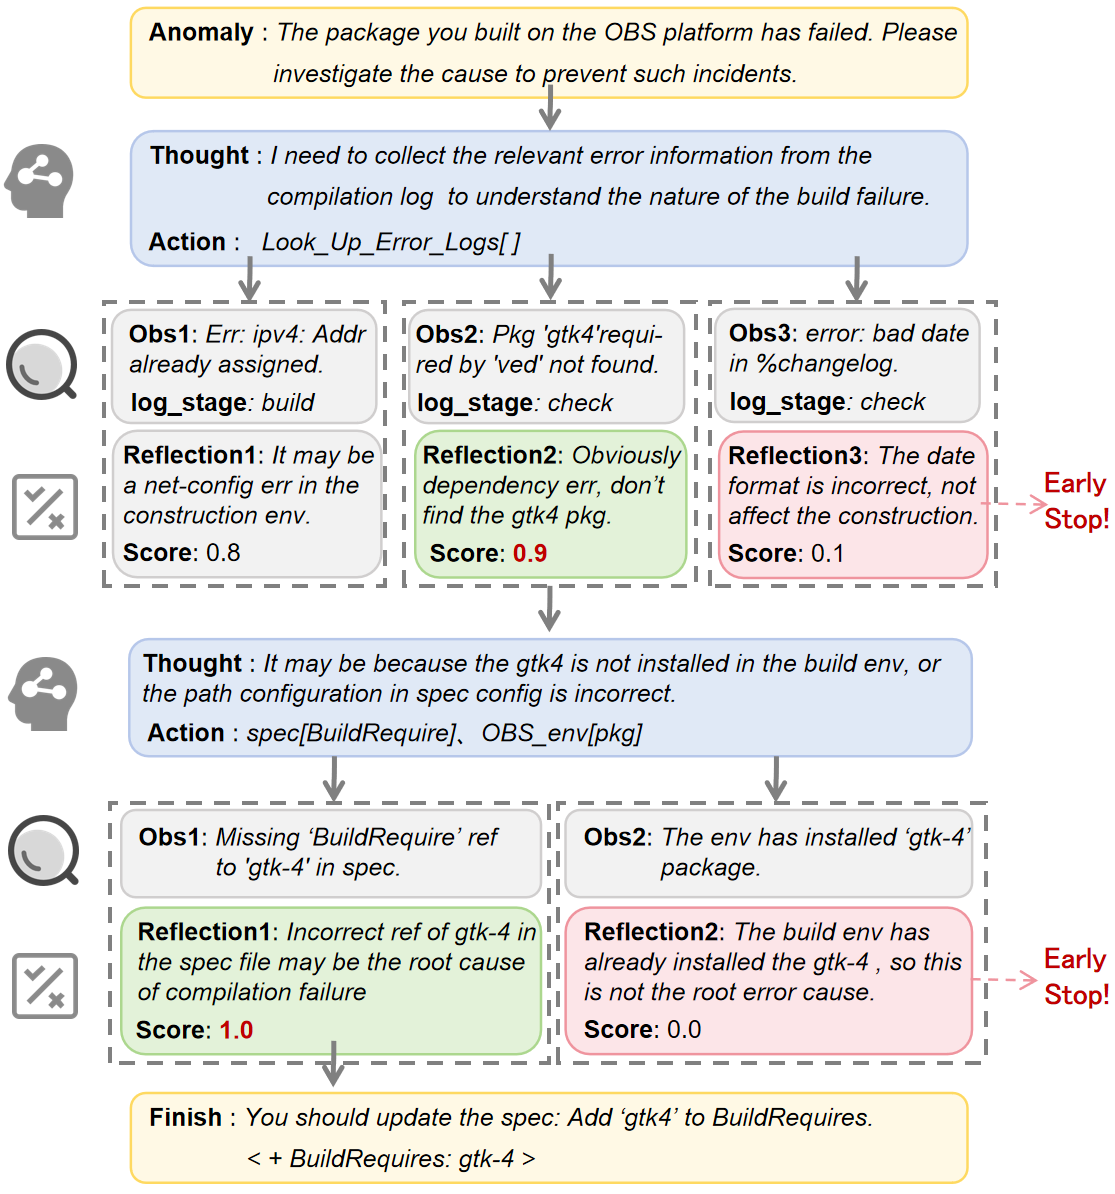
\includegraphics[width=1\linewidth]{pic/new-mcts-tree-exp.png}
    \caption{Illustrative Search Path of the MCTS-RCA}
    \label{fig:mcts-tree}
\end{figure}

\subsubsection{Reasoning Process}\label{ss:mcts-reason}
The overall process of MCTS-RCA includes five stages: initialization, selection, expansion, simulation, and backtracking, as shown in Figure~\ref{fig:mcts-overview}. The detailed introduction of each stage is as follows: (1) In the initialization stage, initial queries and ambiguous responses are generated based on the current software package name, construction environment, and other information (such as "currently unable to solve, more relevant information needs to be obtained") to establish root nodes and minimize overfitting trend of the model. (2) In the selection stage, the algorithm uses a value function Q to rank all non leaf nodes, and uses a greedy strategy to select the node with the highest value for further exploration. (3) In the expansion phase, unless the final destination node is in a termination state, the child nodes of the selected node are expanded by selecting an operation and creating a new node using the operation result. (4) During the simulation phase, the algorithm performs random simulations starting from a new node until it reaches a termination state. (5) During the backtracking phase, the values of the nodes are backpropagated to the root node, and the values of each node are updated with expected values along the way. Figure~\ref{fig:mcts-tree} shows a illustrative search path of the MCTS-RCA.

\subsubsection{Self-Consistency Node Evaluation}\label{ss:mcts-selfcons}
In order to improve the accuracy of node evaluation, MCTS-RCA introduced a node evaluation method based on LLM self consistency. After generating new tree nodes, the system needs to rate their potential value and select the node with the highest score as the target for subsequent expansion. In order to fully utilize the prior knowledge of error categories, this paper improves the traditional UCT evaluation algorithm and proposes a classification-constrained UCT formula:
\begin{equation}
\mathrm{CC}-\mathrm{UCT}(s) = \mathrm{V}(s) + \mathrm{P}(s) \cdot w \cdot \sqrt{\frac{\ln N(p)}{N(s)}}
\end{equation}

V(s) represents the value rating function of the node, P(s) is the confidence weight based on the error category, N(s) is the number of visits to the node, w is the exploration weight, and p is the parent node of the node. In order to better adapt the MCTS-RCA method to different tasks, the V(s) and P(s) of each node are obtained through dynamic inference during the search process. Under the current scoring mechanism, subnodes with low correlation to the error category of the current inference path will receive lower P(s) weights, resulting in lower UCT scores, and thus impose category constraints on the inference path of MCTS. However, this evaluation criterion does not directly prune inference paths with low class relevance, preserving the completeness of the inference space and to some extent avoiding the omission of optimal solutions.

\subsubsection{Termination Conditions}\label{ss:mcts-term}
The termination strategy of MCTS-RCA balances the dual goals of efficiency and completeness, and includes the following two core conditions. When either condition is met, the algorithm will terminate the search: (1)Early termination mechanism: When the LLM outputs a predefined termination identifier during the "think action" generation stage (such as "[success] construction failure reason is openssl version incompatibility"), the system immediately terminates the current search and returns the inference result of the successful node. (2)Maximum simulation count constraint: If the algorithm fails to meet the early termination condition within the maximum simulation count (e.g. 20 steps), the system will automatically terminate the search and output the leaf node with the highest benefit score as the final result. 

This termination mechanism not only avoids meaningless over searching, but also provides reliable backup solutions in complex scenarios.

\section{EXPERIMENTAL EVALUATION}

The experimental design revolves around the problem of software package construction in actual production environments, with a focus on evaluating the performance of the method in different scenarios, including accuracy, module contribution, and adaptability to multiple Large Language Models (LLMs). By comparing with existing baseline methods, further demonstrate the superiority of the proposed method in complex log analysis tasks.
\begin{itemize}
\item RQ1:How accurate is the method in root cause analysis?
\item RQ2:How capable is the method in recommending candidate root causes?
\item RQ3:How does the method enhance the reasoning ability of large language models (LLMs)?
\item RQ4:How accurate is the method in log anomaly detection?
\end{itemize}

\subsection{Experimental Setup}\label{sec:exp-setup}

\subsubsection{Datasets}\label{ss:exp-datasets}
The experiment is based on the open-source software building platform Open Build Service (OBS). The dataset is collected from the real production environment of OBS and includes repair materials for software package construction failure cases (such as error logs, spec files, build environment metadata, etc.). Among them, the original construction logs are processed by the log anomaly detection module to form semantically aligned JSON format log blocks as input for root cause analysis; The root cause of the error is annotated by professionals with over two years of OBS maintenance experience to ensure the reliability of the annotated results. As shown in Figure~\ref{fig:dataset}, the final dataset covers 117 typical construction failure cases, including common problem types such as missing dependencies, configuration conflicts, and compilation errors, etc.

\begin{figure}
    \centering
    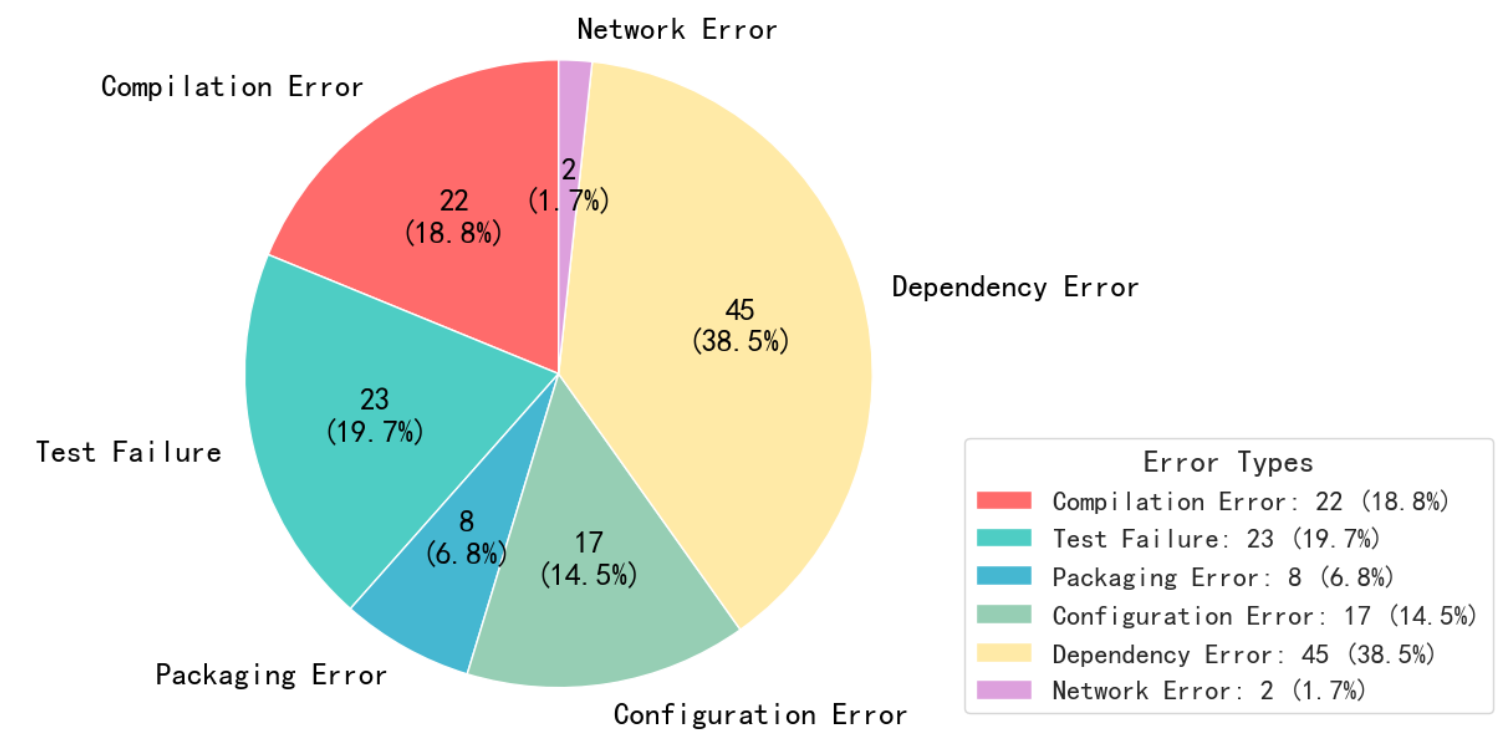
\includegraphics[width=1\linewidth]{pic/dataset-530.png}
    \caption{Proportional Analysis of Error Categories in RISC-V Build Dataset}
    \label{fig:dataset}
\end{figure}



\subsubsection{Baselines}\label{ss:exp-baselines}
To validate the effectiveness of the proposed method, this paper selected multiple baseline methods for comparative experiments. First, the pure LLM generation approach directly inputs relevant build materials into a large language model (LLM) to generate root cause analysis results. Second, the Retrieval-Augmented Generation (RAG) method enhances the LLM's contextual understanding by retrieving a few historical cases from the MCTS-RCA knowledge base as prompts through retrieval augmentation techniques. 

Additionally, this paper compares three LLM-based reasoning frameworks:
(1) ReAct Reflection Framework : ReAct iteratively refines its analysis by integrating external tool calls and internal reasoning steps. However, its high complexity may lead to increased inference time, utilizing the same toolset as MCTS-RCA.
(2) Chain-of-Thought (CoT) : CoT improves result interpretability by explicitly articulating reasoning chains but faces performance limitations when handling multi-source information fusion.
(3) Tree-of-Thought (ToT) : ToT simulates human divergent thinking by constructing multi-branch reasoning paths and supports parallel exploration of candidate solutions. Unlike MCTS-RCA, ToT does not validate intermediate conclusions through tool calls during inference.
By comparing with these baseline methods, this paper demonstrates the superiority of the proposed method in accuracy, efficiency, and applicability.

\subsubsection{Evaluation Metrics}\label{ss:exp-metrics}
This study evaluates the method's root-cause identification capability through multi-dimensional metrics across three dimensions: accuracy, ranking performance, and reasoning effectiveness. These metrics ensure scientific validity by assessing practical applicability from multiple perspectives.Precision, Recall, and F1-score quantify exact error localization capability under strict matching criteria. The F1-score (harmonic mean of Precision and Recall) provides balanced performance evaluation.
% \begin{equation}
% F1 = 2 \cdot \frac{\text{Precision} \cdot \text{Recall}}{\text{Precision} + \text{Recall}}
% \end{equation}

These quantify the method's ability to rank candidate root causes, focusing on inclusion of true root causes in the ranked list. The TOP-K hit rate quantifies the proportion of test cases where true root causes appear within the top K positions, assessing coverage under constrained manual verification. Formula as:

\begin{equation}
\text{TOP-K} = \frac{1}{N} \sum_{i = 1}^{N} \mathbb{I} \left( \text{correct root cause} \in \text{top } K \text{ items} \right)
\end{equation}

\subsubsection{Implementation Details}\label{ss:exp-impl}
In this experiment, two large-language models, GLM-4 and DeepSeek-R1, are used as the reasoning bases. All models are invoked online through the official API interfaces. To ensure the fairness of the experiment, the core parameters are uniformly configured as follows: $temperature = 0$ (to ensure deterministic output), $max_tokens = None$ (to place no limit on the output length), and $timeout = None$ (to avoid interference from timeouts).


In the "accuracy assessment experiment" and the "analysis experiment on the ability to recommend candidate root causes", all comparative methods use GLM-4 as the unified reasoning base. The method of controlling variables is adopted to eliminate the influence of model differences on the results. In the "reasoning ability assessment experiment", a horizontal comparison experiment involving GLM-4 and DeepSeek-R1 is carried out. During the experiment, the two models maintain strict consistency in key parameters such as the maximum concurrency ($Max Concurrency = 16$) to ensure the validity of the comparison results. 

\subsection{RQ1:How accurate is the method in root cause analysis?}\label{sec:rq1}
In this experiment, the accuracy of the proposed MCTS-RCA method was evaluated and compared with five baseline methods. Compared with the pure LLM method, MCTS-RCA effectively improves the reliability of root-cause analysis by introducing a reasoning mechanism based on Monte Carlo Tree Search (MCTS). In contrast to the RAG method, MCTS-RCA is based on a dynamic tool-calling mechanism, which allows the method to dynamically acquire domain-related knowledge during the reasoning process, thus solving the strong dependence of traditional methods on the quality of prompt samples.

\begin{table}[htbp]
    \centering
    \caption{COMPARATIVE ACCURACY OF ROOT CAUSE ANALYSIS METHODS FOR RISC-V}
    \label{tab:accuracy_results}
    \begin{tabular}{lccc}
        \hline
        Model & Prec & Rec & F1 \\
        \hline
        GLM4 & 0.324 & 0.475 & 0.385 \\
        RAG & 0.616 & 0.594 & 0.605 \\
        CoT & 0.554 & 0.528 & 0.541 \\
        ReAct & 0.578 & 0.642 & 0.608 \\
        ToT & 0.634 & 0.718 & 0.673 \\
        MCTS-RCA & \textbf{0.752} & \textbf{0.836} & \textbf{0.792} \\
        \hline
    \end{tabular}
\end{table}

In the comparison with baseline methods of reasoning framework types, MCTS-RCA integrates a multi-level reasoning mechanism, overcoming the limitations of existing methods. Compared with the CoT framework, MCTS-RCA designs a cross-modal information fusion module, which improves the precision by 19.8\% in the scenario of multi-source log correlation analysis. Compared with the ReAct framework, this method improves the reasoning accuracy through a Monte Carlo Tree Search reasoning process based on classification constraints. Notably, MCTS-RCA further optimizes the decision-path selection strategy on the basis of the ToT framework. By introducing a reasoning-path constraint strategy driven by error categories, it increases the F1-score of the root-cause analysis task by 11.9\%.



\subsection{RQ2:How capable is the method in recommending candidate root causes?}\label{sec:rq2}
This experiment evaluates the effectiveness of different methods in the root-cause ranking task through the Top-K metric. The experimental results show that the MCTS-RCA method significantly outperforms the baseline methods in both Top@1 and Top@5 metrics, verifying its root-cause coverage ability in the scenario of manual review. Compared with other baseline methods, MCTS-RCA greatly improves the Top@5 performance by combining the domain knowledge base with the tree-search reasoning strategy, indicating that the ranking optimization guided by domain knowledge can effectively improve the positioning efficiency of key root causes. In the comparison of reasoning frameworks, the Top@5 hit rate of MCTS-RCA is 8.3\% higher than that of ToT, mainly due to its mechanism that can dynamically obtain relevant construction environment information during the reasoning process, enabling the LLM to capture multi-dimensional features such as log error information and spec configuration information simultaneously for causal reflection.

\begin{table}[htbp]
    \centering
    \caption{Results of the Effectiveness Evaluation of Candidate Root Cause Ranking}
    \label{tab:candidate_root_cause_ranking}
    \begin{tabular}{lcc}
        \hline
        Model & Top@1 & Top@5 \\
        \hline
        GLM4 & 0.324 & 0.594 \\
        RAG & 0.616 & 0.684 \\
        CoT & 0.554 & 0.778 \\
        ReAct & 0.578 & 0.762 \\
        ToT & 0.634 & 0.824 \\
        MCTS-RCA & \textbf{0.752} & \textbf{0.907} \\
        \hline
    \end{tabular}
\end{table}

It is worth noting that the performance of existing methods in the Top@1 metric is generally low, reflecting the challenges of accurately locating a single root cause in complex error scenarios. By introducing a search-constraint strategy based on error categories, MCTS-RCA significantly improves the credibility of the first-item recommendation (8.3\% higher than ToT) while maintaining a high recall rate. This feature enables it to reduce the additional work of manual review in actual operation and maintenance scenarios. When the Top@5 coverage rate reaches 90.7\%, the top 5 analysis recommendations can cover the vast majority of key root causes, significantly reducing the operation and maintenance costs. 


\subsection{RQ3:How does the method enhance the reasoning ability of large language models (LLMs)?}\label{sec:rq3}

\begin{figure}
    \centering
    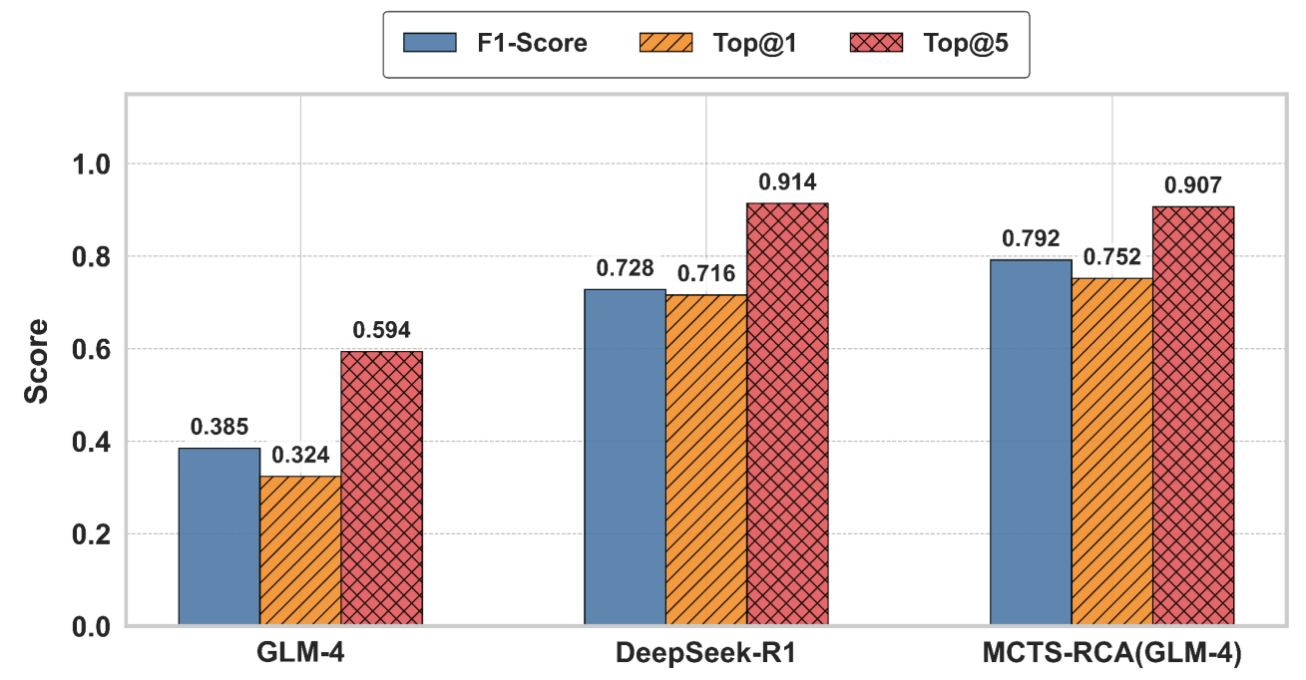
\includegraphics[width=1\linewidth]{pic/reasoning-exp.png}
    \caption{Experimental Results of Reasoning Capability Evaluation}
    \label{fig:reasoning-exp}
\end{figure}

To verify the performance of the method in this paper in terms of reasoning ability, a reasoning evaluation experiment was designed. The root-cause analysis performance of the method based on general large-scale models was compared with that of a professional reasoning model (DeepSeek-R1) to analyze the improvement effect of the method on the reasoning ability of general large-scale models.

As shown in Figure~\ref{fig:reasoning-exp}, the MCTS-RCA method can effectively improve the reasoning ability of general LLMs in the scenario of root cause analysis of RISC-V software package construction errors, with significant increases in both F1-scores and Top@K scores. When compared with the professional reasoning model DeepSeek-R1, it can be found that the method in this paper enables general models to have root-cause analysis capabilities comparable to those of reasoning models. Moreover, its F1-Score leads by 6.4\% and the Top@1 metric leads by 3.6\%, indicating that the method in this paper has obvious reasoning ability in accurately locating the root cause of errors. This may benefit from the introduction of a relevant knowledge base in the field of RISC-V software package construction in the current method, and the enhancement of the LLM's understanding of the relevant field through the method of toolset invocation. 

\subsection{RQ4:How accurate is the method in log anomaly detection?}\label{sec:rq4}

To verify the effectiveness of the method proposed in this paper, the experiment selects three general log anomaly detection methods based on large language models (LLMs) as baseline methods. The core ideas of each baseline method are as follows:

(1) LogGPT is an end-to-end log anomaly detection method based on ChatGPT. Its core lies in utilizing the language understanding ability of ChatGPT to parse the original logs into structured sequences and construct compound prompts.

(2) RAGLog is based on the Retrieval-Augmented Generation (RAG) framework, which improves the detection accuracy by integrating historical normal log cases. 

(3) LogPrompt focuses on optimizing prompt engineering to enhance the reasoning ability of the LLM. It constrains the log format through input/output control functions and designs a multi-level prompt strategy to guide the LLM to complete the log anomaly detection task. 

\begin{table}[htbp]
\centering
\caption{Performance Comparison of Log Analysis Models}
\small % 缩小字体
\setlength{\tabcolsep}{3pt} % 减小列间距
\begin{adjustbox}{width=\columnwidth,center} % 自动缩放到列宽
\begin{tabular}{l *{9}{S[table-format=1.3]}}
\toprule
\multirow{2}{*}{\textbf{Model}} & 
\multicolumn{3}{c}{\textbf{Total}} & 
\multicolumn{3}{c}{\textbf{Prep\&Install}} & 
\multicolumn{3}{c}{\textbf{Build\&Check}} \\
\cmidrule(lr){2-4} \cmidrule(lr){5-7} \cmidrule(l){8-10}
 & {\textbf{Prec}} & {\textbf{Rec}} & {\textbf{F1}} & 
   {\textbf{Prec}} & {\textbf{Rec}} & {\textbf{F1}} &
   {\textbf{Prec}} & {\textbf{Rec}} & {\textbf{F1}} \\
\midrule
LogPrompt    & 0.521 & 0.928 & 0.667 & 0.873 & 0.997 & 0.931 & 0.451 & 0.914 & 0.604 \\
RAGLog       & 0.601 & 0.935 & 0.732 & 0.912 & 0.982 & 0.946 & 0.539 & 0.926 & 0.681 \\
LogGPT      & 0.503 & 0.948 & 0.657 & 0.832 & \bfseries 1.000 & 0.908 & 0.437 & 0.937 & 0.596 \\
RV-LAD       & \bfseries 0.718 & \bfseries 0.976 & \bfseries 0.827 & \bfseries 0.936 & 0.994 & \bfseries 0.964 & \bfseries 0.674 & \bfseries 0.972 & \bfseries 0.796 \\
\bottomrule
\end{tabular}
\end{adjustbox}
\end{table}

In this paper, the RV-LAD method (the RISC-V software package construction log anomaly detection method proposed in this paper) is compared with other baseline methods through experiments on the same dataset. The F1 score of the RV-LAD method is higher than that of other methods, and its accuracy is significantly higher than that of other methods. This indicates that the RV-LAD method has high accuracy and reliability in detecting log anomalies. For the logs in the prep and Install stages, the accuracy of each method is relatively high. This is because the logs in these two stages have similar structures and lower complexity, so they are more likely to be accurately classified. However, for the logs in the Build and Check stages, the accuracy of all methods decreases. This may be due to the diverse structures, complex semantics, and more noise interference of the logs in these two stages, making it difficult for the model to distinguish between normal and abnormal data. 


\section{Bad Case Study}

We conducted additional analysis on the experimental results of log root cause analysis based on error types. The recognition accuracy of each type is as follows: compilation error recognition accuracy is 68.18\%, test failure recognition accuracy is 69.56\%, build error recognition accuracy is 87.5\%, configuration error recognition accuracy is 100\%, dependency error recognition accuracy is 95.55\%, and network problems are basically not recognized.
Through the analysis of typical misjudgment samples, we find two main issues:

(1) There is ambiguity in the annotated data. The boundary between "network problem-download failure of dependency library" and "dependency error-lack of dependency" is blurred and easily misjudged. The sample size of this type of problem is relatively small, with only two instances, both of which result in build errors due to the inability to download dependencies from Huawei Cloud images (huaweicloud. com).
For example, the key error message for \textit{jaxb2-common} bases is  \textit{"Could not resolve dependencies for project org. jvnet. jaxb2-commons: jaxb2-bbases: jar: 0.9.5"}, but our method misjudges it as a "dependency error", which is actually due to network reasons causing the failure to obtain dependencies.

(2) Multi-stage composite error localization problem. In the categories of "compilation errors" and "test failures", there are composite errors with multiple stages and languages, making it difficult to locate key errors. This error spans multiple build stages (prep, install, build, check), with more than 10 error blocks and involving two or more programming languages (C, Go, Java, Python). The error propagation chain is long and there is a lot of interference information, making it difficult for the model to accurately extract key features.
For example, the error source of libaio is that the C++dependency library for Python library encodings failed to compile successfully. Our method identifies the intermediate error message "groupadd" command not found as a key feature, resulting in a misjudgment as "dependency missing" and failing to recognize that it actually belongs to a "compilation error".
This case reflects that there is still significant room for improvement in key error localization and contextual modeling when facing complex construction failures across languages and stages.


\section{CONCLUSION}
This paper presents a two-stage framework for diagnosing RISC-V build failures: RV-LAD distills phase-aware log evidence via template-based filtering, and MCTS-RCA performs tool-augmented, knowledge-guided reasoning to identify root causes with interpretable traces. 
Experimental results on real-world OBS build failures demonstrate that our approach outperforming existing LLM-based methods across multiple metrics. Furthermore, the proposed framework significantly enhances the reasoning capability of general-purpose LLMs and provides interpretable decision traces to support developer debugging. Our framework is designed with a clear separation between a domain-agnostic core and customizable domain plug-ins, allowing it to generalize beyond RISC-V with minimal changes.

In future work, we will develop developer-facing tools (e.g., IDE/CI plugins) to ease adoption in real workflows. We will also collect  usage feedback and troubleshooting traces to continually refine prompts, knowledge bases, and tools, improving robustness and generalization.


% \begin{thebibliography}{00}
% \bibitem{b1} G. Eason, B. Noble, and I. N. Sneddon, ``On certain integrals of Lipschitz-Hankel type involving products of Bessel functions,'' Phil. Trans. Roy. Soc. London, vol. A247, pp. 529--551, April 1955.
% \bibitem{b2} J. Clerk Maxwell, A Treatise on Electricity and Magnetism, 3rd ed., vol. 2. Oxford: Clarendon, 1892, pp.68--73.
% \bibitem{b3} I. S. Jacobs and C. P. Bean, ``Fine particles, thin films and exchange anisotropy,'' in Magnetism, vol. III, G. T. Rado and H. Suhl, Eds. New York: Academic, 1963, pp. 271--350.
% \bibitem{b4} K. Elissa, ``Title of paper if known,'' unpublished.
% \bibitem{b5} R. Nicole, ``Title of paper with only first word capitalized,'' J. Name Stand. Abbrev., in press.
% \bibitem{b6} Y. Yorozu, M. Hirano, K. Oka, and Y. Tagawa, ``Electron spectroscopy studies on magneto-optical media and plastic substrate interface,'' IEEE Transl. J. Magn. Japan, vol. 2, pp. 740--741, August 1987 [Digests 9th Annual Conf. Magnetics Japan, p. 301, 1982].
% \bibitem{b7} M. Young, The Technical Writer's Handbook. Mill Valley, CA: University Science, 1989.
% \end{thebibliography}
\vspace{12pt}

\bibliographystyle{IEEEtran}
\bibliography{reference}
\end{document}
